\vspace{0.5cm}
\begin{center}
    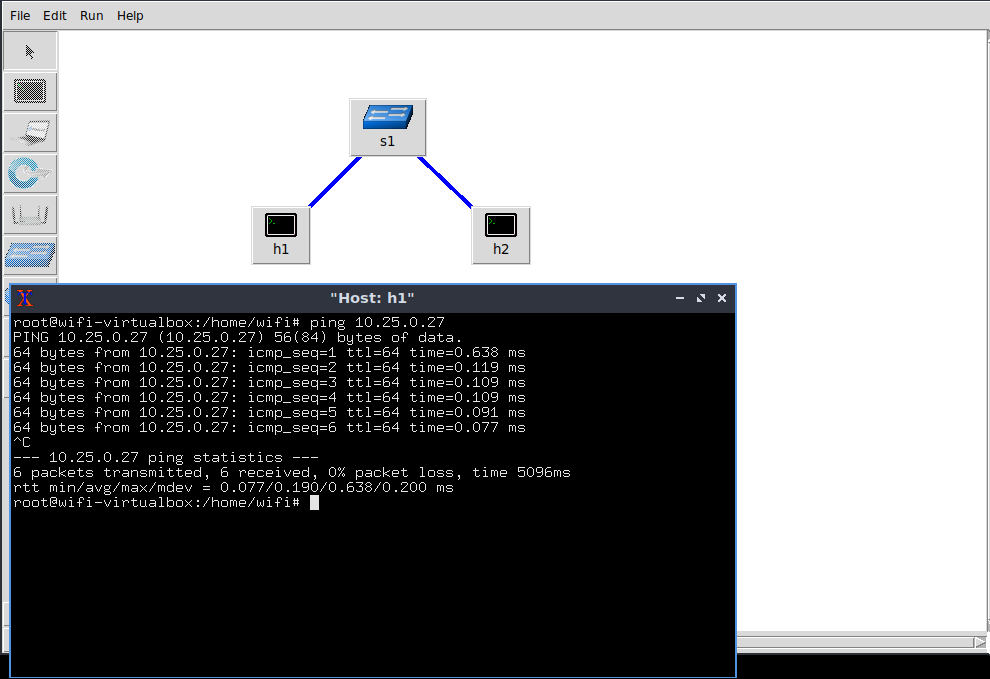
\includegraphics[width=1\textwidth]{./images/T1.2TopologyAndPing.png}
\end{center}
\textbf{1:} `tc qdisc add dev h2-eth0 root netem rate 125mbit`
\begin{center}
    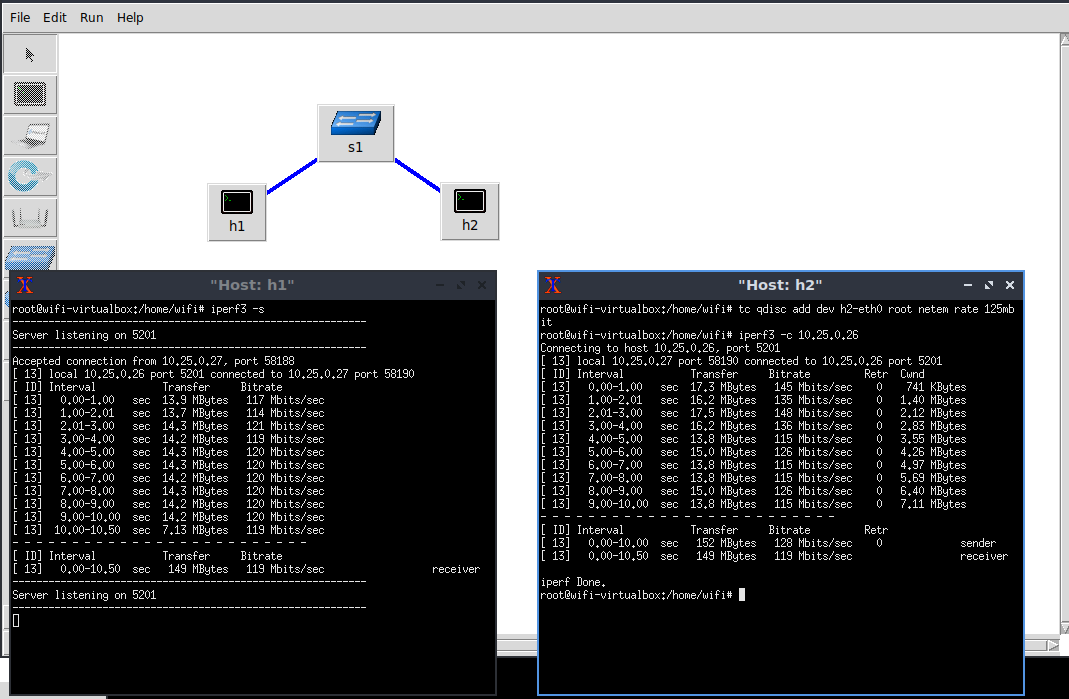
\includegraphics[width=1\textwidth]{./images/T1.2/125test2.png}
    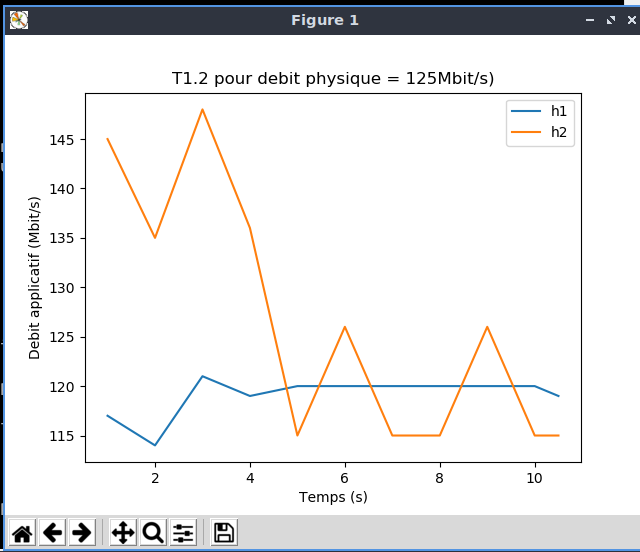
\includegraphics[width=1\textwidth]{./images/T1.2/courbe125test2.png}
    
\end{center}
\textbf{Observation :}\\
Débit de H1 (ligne bleue) : Le débit applicatif mesuré sur h1 reste relativement stable, oscillant entre 115 Mbit/s et 125 Mbit/s tout au long du test. Même si le lien physique entre H1 et le switch est de 1 Gbit/s, le débit observé n’atteint jamais cette valeur maximale théorique.

Débit de H2 (ligne orange) : Le débit applicatif de H2 fluctue considérablement, atteignant parfois des pics autour de 145 Mbit/s, mais chutant aussi à des valeurs proches de 120 Mbit/s ou même légèrement en dessous.
\vspace{1cm}
\\
\textbf{Explications :} 
\\
Bien que la liaison entre h1 et le switch soit fixée à 1 Gbit/s, c'est le lien entre H2 et le switch qui impose une limite plus contraignante de 125 Mbit/s.\\
Dans ce type de configuration, le débit total du transfert est dicté par le maillon le plus faible de la chaîne, en l’occurrence la connexion limitée entre H2 et le switch. Le lien de 1 Gbit/s entre h1 et le switch ne peut donc pas être exploité pleinement tant que H2 ne peut pas recevoir ou envoyer des données plus rapidement que 125 Mbit/s.\\
\\
L'outil iperf3 utilise généralement le protocole TCP, qui ajuste automatiquement le débit en fonction des capacités du réseau. TCP surveille les capacités des deux hôtes et ajuste son débit en fonction des retours qu’il reçoit (accusés de réception des paquets).
Ici, TCP détecte que le débit sur le lien entre H2 et le switch est limité à 125 Mbit/s et ajuste donc la transmission des données pour s’adapter à cette contrainte, expliquant pourquoi le débit de h1 reste autour de 115 à 125 Mbit/s.
Le protocole TCP est conçu pour éviter la surcharge du réseau et s’adapte dynamiquement aux conditions de congestion, ce qui pourrait aussi expliquer pourquoi le débit de H2 est plus instable, car le lien est proche de sa capacité maximale.\\
\\
\textbf{2:} `tc qdisc add dev h2-eth0 root netem rate 625mbit `
\begin{center}
    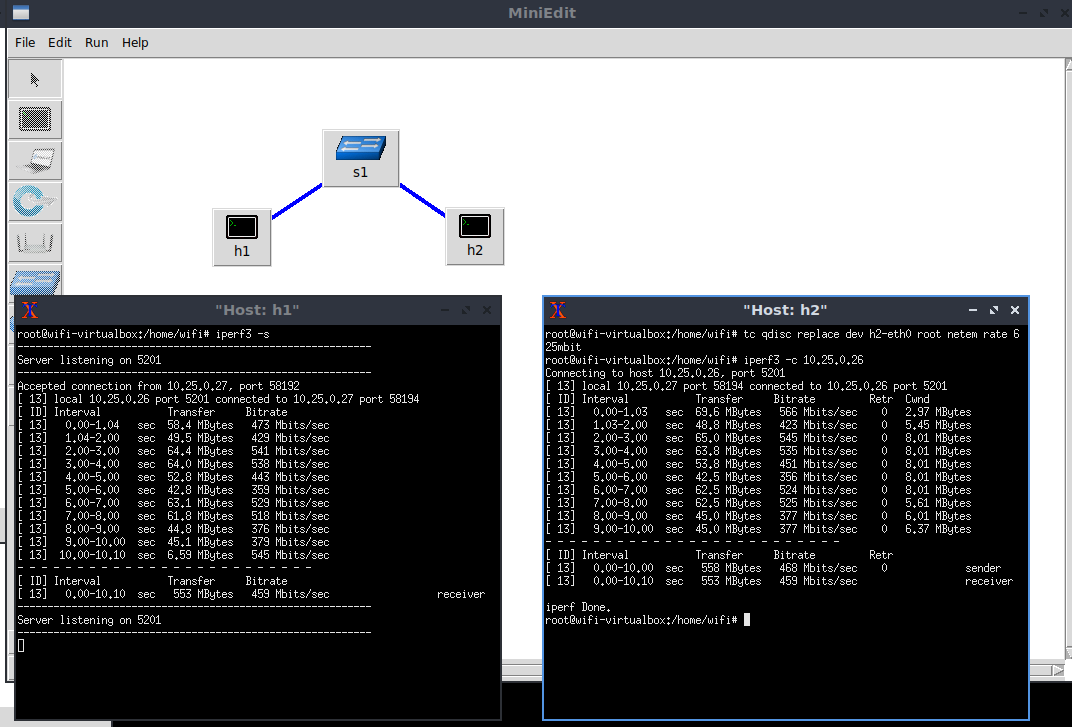
\includegraphics[width=1\textwidth]{./images/T1.2/625test2.png}
    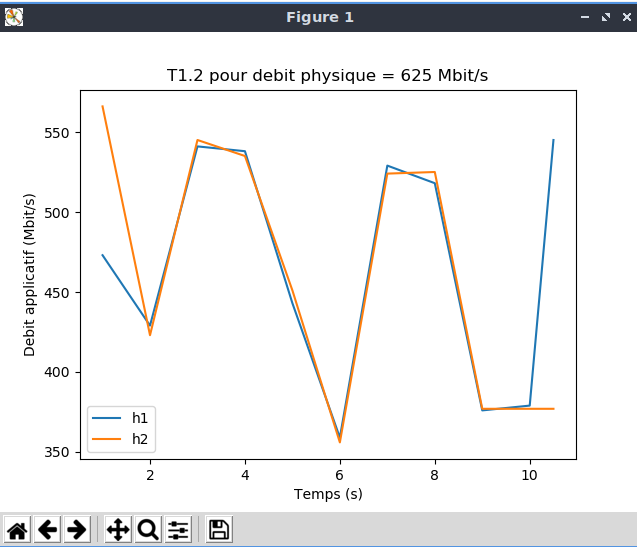
\includegraphics[width=1\textwidth]{./images/T1.2/courbe625test2.png}
\end{center}
\textbf{Observation :}\\
Débit de h1 (ligne bleue) : Le débit applicatif mesuré sur h1 varie entre 350 Mbit/s et environ 550 Mbit/s.
Débit de h2 (ligne orange) : Le débit applicatif sur H2 suit une courbe similaire à celle de h1.
\\
\textbf{Explication} :\\
Le fait que les deux débits (h1 et h2) suivent un schéma similaire de montée et descente suggère que la limitation du débit physique à 625 Mbit/s entre H2 et le switch influence directement les deux hôtes. Comme le débit de H2 est limité par le lien physique, le switch agit comme un point de congestion, entraînant des fluctuations du débit applicatif.
\vspace{1cm}
\\
\textbf{3:} `tc qdisc add dev h2-eth0 root netem rate 2.5gbit`
\begin{center}
    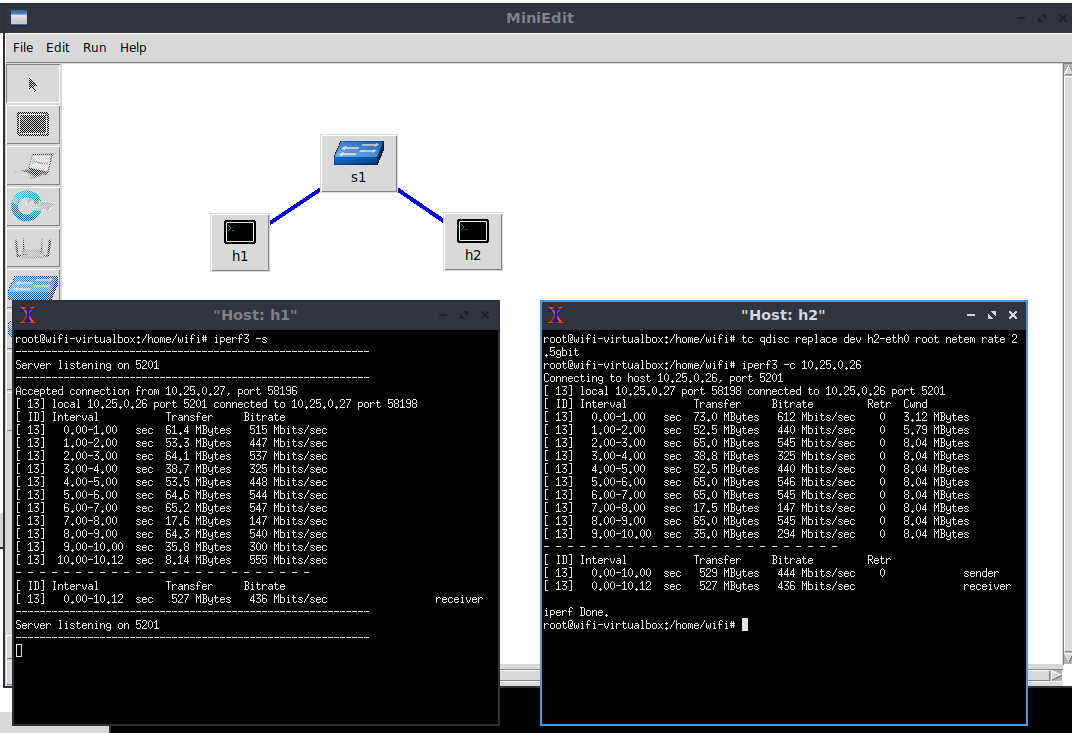
\includegraphics[width=1\textwidth]{./images/T1.2/2500test2.png}
    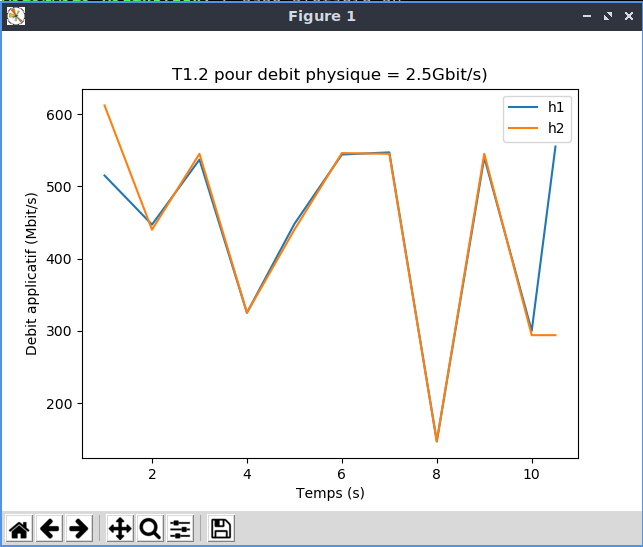
\includegraphics[width=1\textwidth]{./images/T1.2/courbe2500test2.png}
\end{center}

\newpage
\textbf{Courbe T1.2:} 




